\chapter{微分\&链式法则}

\begin{figure}[ht]
  \centering
  \includegraphics[width=1\linewidth]{asset/茶桁的 AI 秘籍_Math_10.png}
\end{figure}

\newpage

我们上节课讲了导数. 今天将会是两部分, 一部分是「微分」, 一部分是「链式法则」. 

\section{微分}

微分, 我们在导论里面提过. 它和导数比较像, 但是还是有差别的. 实际的定义和内容都比较简单, 我们先来看看定义:

\begin{align*}
  & \mbox{当自变量 x 的变化趋于无穷小时}(dx), \mbox{因变量}f(x)\mbox{的变化情况}(df(x)) \\
  & df(x) = f'(x)dx
\end{align*}

当自变量$x$的变化趋于无穷小的时候,我们用$dx$来表示. 因变量$f(x)$的变化情况, 我们用$df(x)$来表示, 在这里$df(x)$等于$f'(x)dx$. 

所以微分它和导数是不一样的. 导数是什么?是函数在某一点的\textbf{变化率}, 是$\frac{df(x)}{dx}$. 微分呢, 是函数在某一点的\textbf{变化量}, 所以一个是\textbf{变化率}一个是\textbf{变化量}. 这就是它们唯一的区别. 

那他们之间有什么联系?我们说: 函数的变化量与自变量变化量之比, 即为导数. 

\begin{align*}
  \frac{df(x)}{dx} = f'(x)
\end{align*}

这些都是从式子得来的, 没什么复杂的地方, 那微分就是这样, 没有更多的内容了. 

接下来, 我们要来学习一个比较重要的概念, 就是链式法则. 

\section{链式法则}

「链式法则」为什么重要. 我们知道神经网络不是只有一层或者两层, 它是有很多层. 比如, 何凯明等人在 2015 年提出的 ResNet, 那个网络就有 152 层. 后来据说这些网络可以上到 1,000 层, 太可怕了. 

我们通过上一节课的动图演示, 知道了是怎么样优化的. 就是通过求导, 然后一步一步的去逼近最小值点去做的. 那问题就来了, 求导只是一层的关系, 后面几层的这些导数怎么传到前面几层?这里就对应着嵌套函数的问题. 

什么叫嵌套函数?就是函数里面套上函数. 

打个比方: $y=f(x)$, $x=g(z)$, $x$又是关于$z$的一个函数. 所以, 我们把它写成一个复合函数的形式, 或者说把$y$用 z 当作自变量来表示:

\begin{align*}
  \mbox{嵌套函数:}& \\
  & y = f(x), x = g(z) \quad \Rightarrow \quad y = f(g(z))
\end{align*}

就是说$f$里面再套一层$g$,然后是$z$. 

好, 我们这个时候来思考一下, 它里面隔着两层函数, 我们怎么样求$y$相对于$z$的一个导数呢? 在这里就需要通过链式法则. 链式法则是怎么得来的?这里一步一步的给大家讲, 先看完整推导式:

\begin{align*}
  y'_z & = \frac{dy}{dz} = \frac{dy}{dz} \cdot 1 = \frac{dy}{dz} \cdot \frac{dx}{dx} = \frac{dy}{dx} \cdot \frac{dx}{dz} \\ \\
  & = f'(x)g'(z) = f'(g(z))g'(z)
\end{align*}

首先,按照导数定义 $y$ 相对于 $z$ 的导数,那就是 $\frac{dy}{dz}$.

然后我们乘以一个 1, 它还是不变. 接下来把 1 可以转化为 $\frac{dx}{dx}$. 

之后将分母调换一下, 把$dx$换过来, 然后把$dz$拿到另外一边去. 通过这么一步变换, 我们就得到 $\frac{dy}{dx} \cdot \frac{dx}{dz}$. 

这一步之后, 现在我们可以套导数定义, 我们惊奇的发现, $\frac{dy}{dx}$不就是$f'(x)$, 而$\frac{dx}{dz}$也正好就是$g'(z)$. 这一步, 是因为$x=g(z)$, 所以$\frac{dx}{dz}$就是函数$g(z)$的导数. 

所以最后, 我们就得到了$f'(x)g'(z)$, 原来$y$隔着一层相对于$g(z)$的导数可以写成$f'(x)g'(z)$的形式. 那我们已知$x=g(z)$,  那我们最后就可以得到$f'(g(z))g'(z)$, 它是中间隔着一层的这么一个关系. 

就是嵌套函数求导的一个方法. 而且不管你有多少层, 你套 100 万层, 只要它是可导的你都可以这样去做. 方法概括一下, 就是先外层求导, 然后再内层求导. 

我们再来看一个例子:

\begin{align*}
  \mbox{例}:& y = x^2, x=e^z, \mbox{求 y 相对于于 z 的导数} \\
\end{align*}

让我们求函数$y=x^2$, $x=e^z$, 然后求$y$相对于$z$的导数. 

$y$关于$z$的导数怎么求? 我们来看:

\begin{align*}
  y'_z & = \frac{dy}{dx} \cdot \frac{dx}{dz} = (x^2)'(e^z)' \\
  & = 2x \cdot e^z = 2e^z \cdot e^z = 2e^{2z}
\end{align*}


套用刚才得到的那个结论, $y'_z$ 就等于$\frac{dy}{dz}$乘以$\frac{dx}{dz}$, 让我们先做外面一层的导数, 再做里面一层的导数. 

外面一层是$x^2$, 然后里面一层是$e^z$. 求出来之后是$2x\cdot e^z$. 

因为我们是求$y$关于$z$的导数,所以我们结果里面不应该出现$x$. 所以我们再把$x$换成用$z$表示的形式. 那很多人就觉得做到这一步就可以了, 但是我们在这里需要把$x$也用 z 来表示一下, 最终结果应该是$2e^2z$. 

如果嵌套 n 多层呢, 如果是非常复杂非常复杂, 一直到$x_n = f_{n-1}(x_{n-1})$, 在这么一个映射法则之下会怎么样呢? 

\begin{align*}
  \mbox{如果嵌套 N 多层...} & \\
  & x_2 = f_1(x_1), x_3 = f_2(x_2), ..., x_n = f_{n-1}(x_{n-1}) \\ \\
  & \frac{dx_n}{dx_1} = \frac{dx_n}{dx_{n-1}} \cdot \frac{dx_{n-1}}{dx_{n-1}} \cdot ... \cdot \frac{dx_2}{dx_1}
\end{align*}

如果是这样, 那也仍然是一样的, 就是逐层求导. 

大家在课后或者复习的时候再看一看链式法则. 它是非常精妙的一个东西, 虽然简单, 但是神经网络的反向传播、后面的这些误差怎么样传播到前面的这些层就靠链式法则, 没有它就不行. 

而且, 链式法则看上去很简单, 但是它的真面目就是我一再强调的\textbf{神经网络的优化原理}、\textbf{反向传播的基石}. 我们看图\ref{fig:img11_1}:

\begin{figure}[ht]
  \centering
  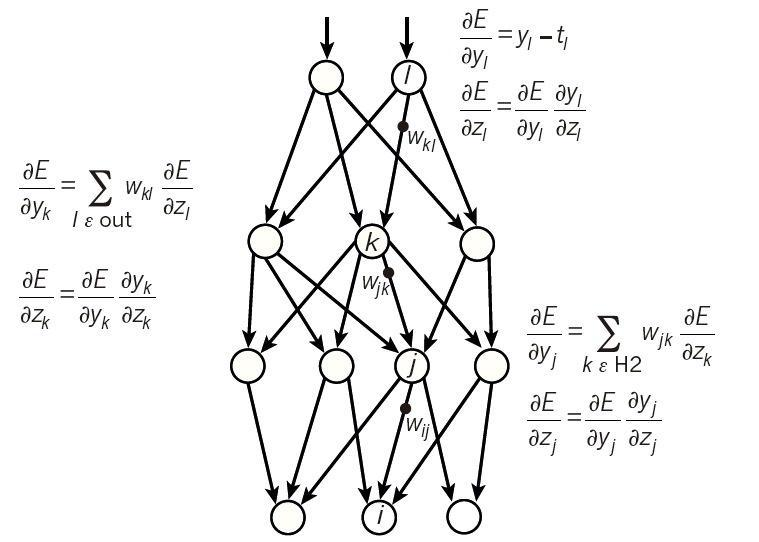
\includegraphics[width=0.8\linewidth]{asset/20200603174921-1878265324_jpeg_759_542_46786.jpg}
  \caption{}
  \label{fig:img11_1}
\end{figure}

这张图上有很多让人头晕的符号, 我们不用去管, 就知道是怎么回事就行. 

就是上面这些层的误差是不断的求导, 通过链式法则传播到前面. 每一层与每一层之间就相当于嵌套了一层函数, 就像我们刚才说的嵌套函数一样. 

本节课我们稍微提了一下「微分」, 然后着重讲了一下「链式法则」,下节课我们讲一下「偏导数」、「方向导数」. 